\section{Longitudinal control}
\label{longitudinal_control}

\section{Questions}
\label{questions_longitudinal_control}

\begin{enumerate}
\item What is the order of the following transfer function?

\begin{equation}
G(s) = \frac{s-10}{s^2 + 2s +1}
\end{equation}
	\begin{enumerate}
		\item  This is the first order transfer function
		\item This is the second order transfer function
		\item This is the third order transfer function
		\item This is the fifth order transfer function
		\item None of the above
	\end{enumerate}
	
\item What are the poles and zeros of the following transfer function?
\begin{equation}
G(s) = \frac{s^2 +3s-10}{s^2 - 2s -12}
\end{equation}
	\begin{enumerate}
		\item  The poles are -3 and 4; the zeros are 2 and -5
		\item The poles are -4 and 3; the zeros are 5 and -2
		\item The poles are 2 and -5; the zeros are -3 and 4
		\item The poles are 5 and -2; the zeros are -4 and 3
		\item None of the above
	\end{enumerate}
\item What might be your action as a system control engineer if you need to increase the overshoot of a control loop system? (Select all that apply)
	\begin{enumerate}
		\item Increase $K_I$
		\item Decrease $K_I$​
		\item Decrease $K_P$ ​
		\item Increase $K_D$ 
		\item Increase $K_P$​
		\item Decrease $K_D$​
	\end{enumerate}
\item Consider the Mass-Spring-Damper System shown in the figure below.

\begin{figure}[!htb]
\begin{center}
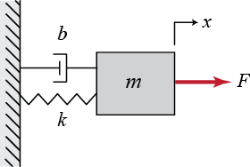
\includegraphics[scale=0.280]{img/longitudinal_control/image_q5_1.png}
\end{center}
\label{image_q5_1}
\end{figure}

As a system control engineer, you constructed the following closed loop transfer function to represent the Mass-Spring-Damper System. 
What is the correct transfer function for this closed loop? 

\begin{figure}[!htb]
\begin{center}
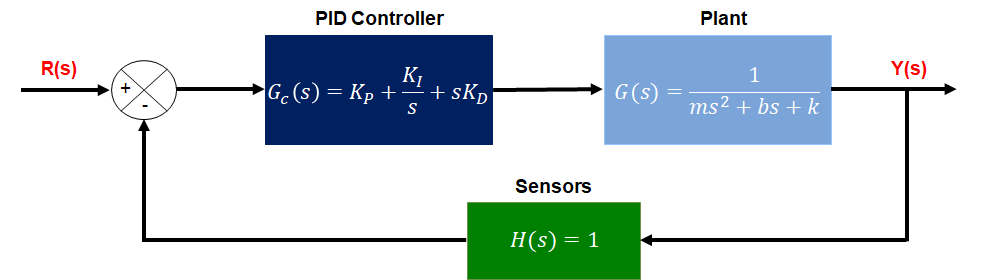
\includegraphics[scale=0.280]{img/longitudinal_control/image_q5_2.png}
\end{center}
\label{image_q5_2}
\end{figure}

\begin{enumerate}
		\item Transformation function 1
		\begin{equation}
			G(s) = \frac{K_Ds^2 + sK_P + K_I}{K_P + \frac{K_I}{s} + K_Ds} 
		\end{equation}
		\item Transformation function 2
		\begin{equation}
			G(s) = \frac{K_P + \frac{K_I}{s} + K_Ds}{K_Ds^2 + sK_P + K_I} 
		\end{equation}
		\item Transformation function 3
		​\begin{equation}
			G(s) = \frac{ms^2 + bs + k + K_P\frac{K_I}{s} + K_Ds}{K_P + \frac{K_I}{s} +K_Ds} 
		\end{equation}
		\item Transformation function 4
		​\begin{equation}
			G(s) = \frac{K_Ds^2 + sK_P + K_I}{ms^3 + (b + K_D)s^2 + (k + K_P)s + K_I} 
		\end{equation}
		\item None of the above
	\end{enumerate}
		
\item You are given the step response of a few different PID controllers using the same gains for the same first order transfer function. 
Determine a possible set of controllers that generated these step responses:

\begin{figure}[!htb]
\begin{center}
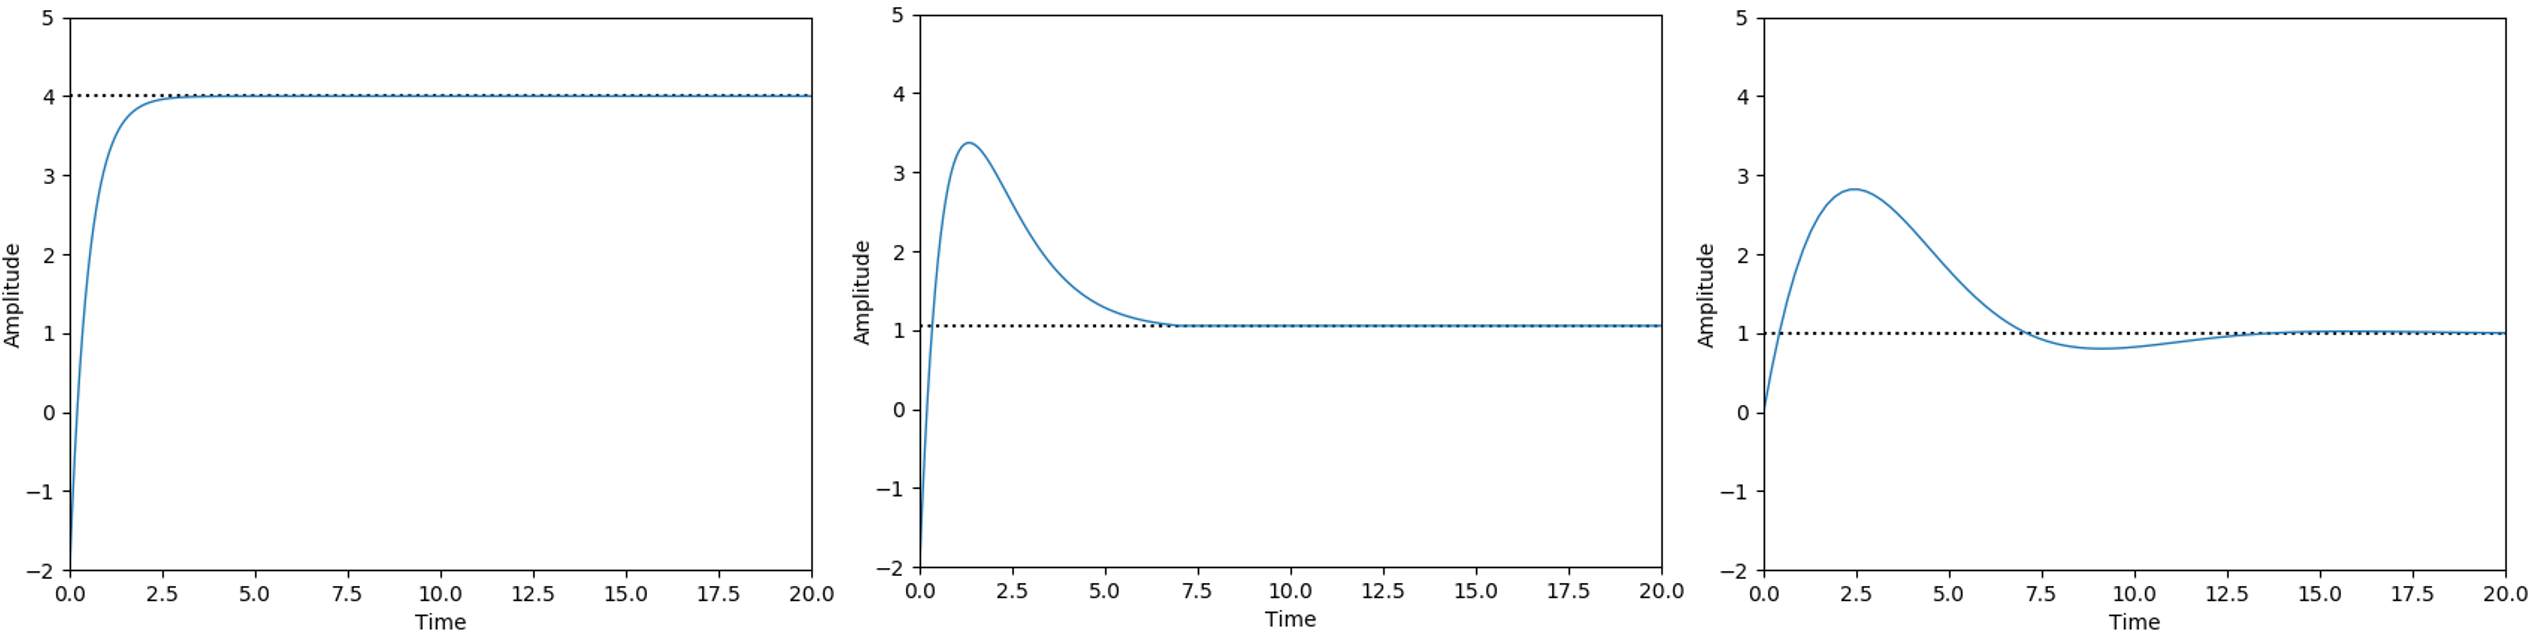
\includegraphics[scale=0.280]{img/longitudinal_control/Full-Size-Image.png}
\end{center}
\label{Full-Size-Image}
\end{figure}

	\begin{enumerate}
		\item 1st response by PI; 2nd response by PD; 3rd response by PID
		\item 1st response by PD; 2nd response by PI; 3rd response by PID
		\item 1st response by PI; 2nd response by PID; 3rd response by PD
		\item 1st response by PD; 2nd response by PID; 3rd response by PI
		\item None of the above
	\end{enumerate}
\item What is the output of a typical output of a Longitudinal control module? (Select all that apply)
	\begin{enumerate}
		\item  Reference velocity
		\item Throttle angle
		\item Steering angle
		\item Brake position
	\end{enumerate}
\item Based on the engine map in the figure below, determine the throttle angle needed to produce 
		250 ft-lb of torque given that the current engine speed is 3500 RPM.
\begin{figure}[!htb]
\begin{center}
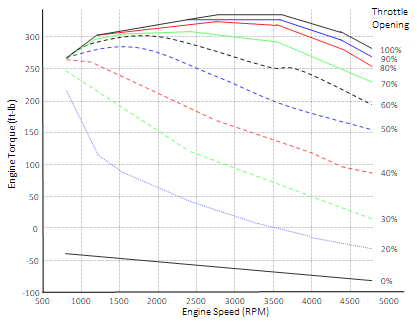
\includegraphics[scale=0.280]{img/longitudinal_control/image_q10.png}
\end{center}
\label{image_q10}
\end{figure}
		
\item The results of a simulation of the control response to a step change in desired speed of a dynamic vehicle model with a PID controller are shown in the figures below. 
There are two spikes on these figures: one spike is between 2 and 3 seconds, another spike is between 3 and 4 seconds. What is the reason of these spikes?
\begin{figure}[!htb]
\begin{center}
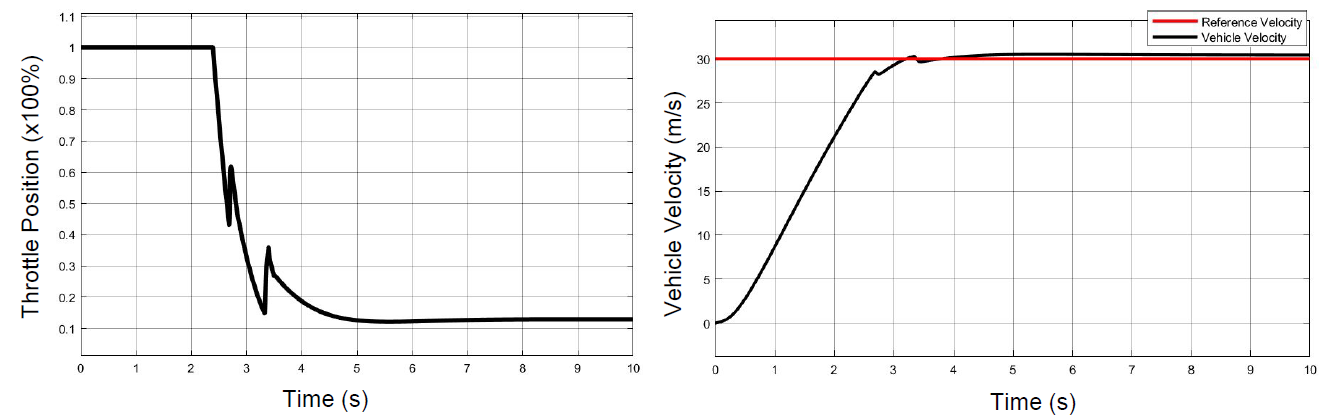
\includegraphics[scale=0.280]{img/longitudinal_control/image_q11.png}
\end{center}
\label{image_q11}
\end{figure}
	\begin{enumerate}
		\item  Engine-transmission torque loss
		\item Tire slip
		\item Nonlinear engine map
		\item High level controller simplification: changing the integral to a summation over fixed length time steps in the Integral term
		\item None of the above
	\end{enumerate}
\item What type of control system is shown in the figure below?
\begin{figure}[!htb]
\begin{center}
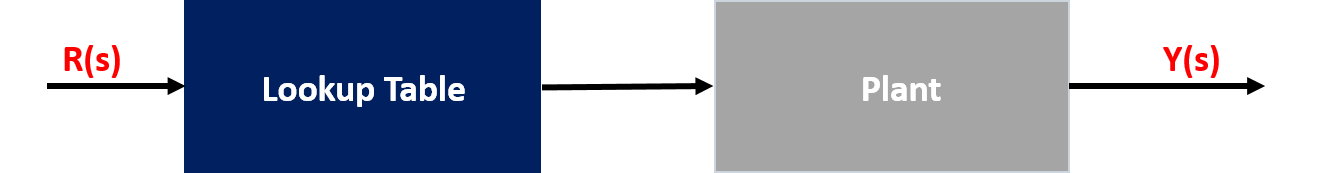
\includegraphics[scale=0.280]{img/longitudinal_control/Openloop.png}
\end{center}
\label{Openloop}
\end{figure}
	\begin{enumerate}
		\item  Feedback control
		\item Feedforward control
		\item Feedback-feedforward control
		\item None of the above
	\end{enumerate}
\item What types of inaccuracies are corrected by a feedback controller?
	\begin{enumerate}
		\item  Disturbances
		\item Nonlinear engine map
		\item Errors in the plant model
		\item High level controller simplification: changing the integral to a summation over fixed length time steps in the Integral term
	\end{enumerate}
\item What assumptions are essential for creation of a longitudinal feedforward input? (Select all that apply)
	\begin{enumerate}
		\item  The tire slip angle and ratio are negligible
		\item The vehicle is at steady state
		\item The plant system is linear
		\item Torque from the engine passes directly to the transmission without loss
	\end{enumerate}
\item What are the sources of the load torque considered for a longitudinal feedforward look-up table computation? (Select all that apply) 
	\begin{enumerate}
		\item   Rolling resistance
		\item Sliding resistance
		\item Gravitational resistance
		\item Cornering force
		\item Aerodynamic resistance
		\item Static friction
	\end{enumerate}
\item A vehicle is being operated on a highway with the reference velocity of $126km/h$ (35 m/s) 
in gear 4 and it overcomes the total load torque of 300 ft-lb. 
This vehicle specification includes effective wheel radius of 0.35 m and 4th gear ratio of 2. 
What throttle angle is required for maintaining the the current speed of the vehicle? Use the below engine map for your computation. 

\begin{figure}[!htb]
\begin{center}
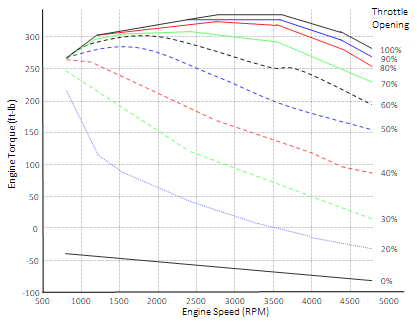
\includegraphics[scale=0.280]{img/longitudinal_control/image_q12.png}
\end{center}
\label{image_q12}
\end{figure}
\end{enumerate}


